\section{Menü-Struktur}\label{sec:menu}

% Siehe auch: https://sopra.informatik.uni-freiburg.de/soprawiki/Men%C3%BC

% Bei der Beschreibung der Menü-Struktur wird erklärt, wie das Hauptmenü und
% alle In-Game-Menüs zueinander in Beziehung stehen. Hilfreich dazu kann ein
% Diagramm in Form eines Graphen oder Baums sein.
%
% Wichtig ist, dass ersichtlich wird, welche Aktion im Menü welche Reaktion des
% Interfaces verursacht. Beispiel: "Wenn man im Einstellungsmenü auf 'Zurück'
% klickt, gelangt man zurück ins Hauptmenü."
%
% Ebenso wichtig ist die Vollständigkeit der Beschreibung. Jedes Menü und jedes
% Untermenü sollten erklärt werden.

\begin{figure}[ht]
	\centering
	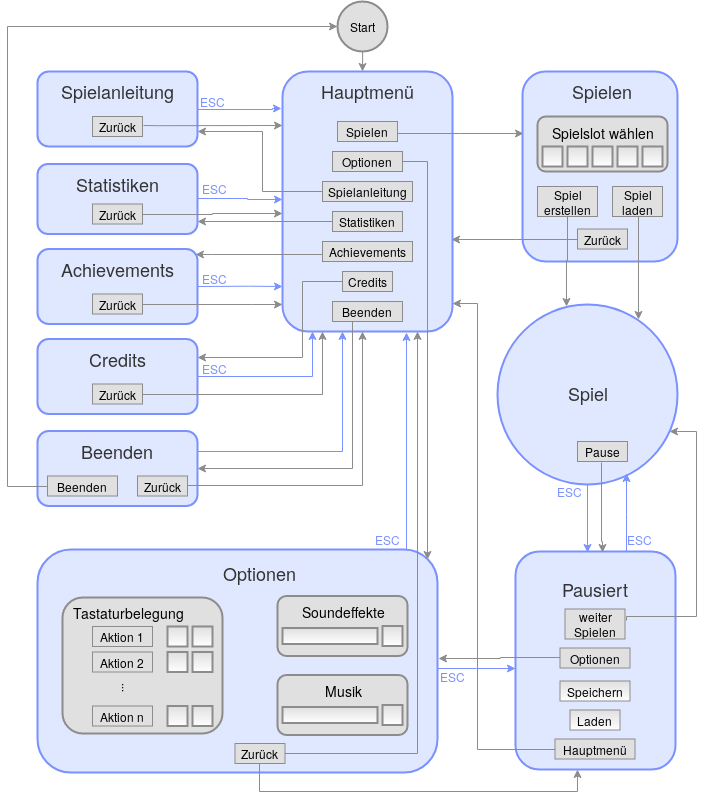
\includegraphics[width=1\textwidth]{menu_structure.png}
  \caption{Die Struktur des Hauptmenüs und des Pausenmenüs in \emph{Kernel Panic!}}
	\label{fig:menu}
\end{figure}

\subsection{Hauptmenü}\label{sec:menu-main}

Beim Starten von \textit{Kernel Panic!} öffnet sich nach der Hintergrundgeschichte direkt das Hauptmenü (siehe Abbildung \ref{fig:menu}). Hier hat man Zugriff auf die \textit{Spielanleitung}, \textit{Statistiken}, \textit{Achievements} und \textit{Credits}.

Durch die Auswahl eines dieser Felder öffnet sich ein Fenster, in dem man diverse
Informationen zum entsprechenden Thema einsehen kann. Mithilfe des Feldes
\textit{Zurück} oder dem Betätigen der \textit{Escape}-Taste gelangt man wieder in das Hauptmenü.\\
Um das Spiel zu beenden wählt man im Hauptmenü das Feld \textit{Beenden}. Damit man nicht versehentlich das Spiel schließt öffnet sich zunächst noch ein zusätzliches Fenster, man kann nun entweder das Beenden bestätigen oder zurückkehren.

Das Feld \textit{Spielen} öffnet das Menü, dass für das Erstellen und das Laden des Spieles zuständig ist. Wenn man nicht durch Wählen der Escape-Taste oder Betätigen des \textit{Zurück}-Feldes das Hauptmenü öffnet, wählt man hier einen von fünf Spielständen, sogenannten \textit{Spielslots}. Jeder \textit{Spielslot} kann entweder genau einen zuvor gespeicherten Spielstand enthalten oder leer sein.

Wenn man einen nicht-leeren \textit{Spielslot} ausgewählt hat kann man
ein angefangenes \textit{Spiel laden} oder ein \textit{Spiel erstellen}; falls
der gewählte \textit{Spielslot} leer ist, bleibt nur die Option, ein neues Spiel zu erstellen.
Unabhängig davon ob der \textit{Spielslot} frei ist, gelangt man nun in das Spiel.


\subsection{Pausenmenü}\label{sec:menu-pause}

Während des Spiel kann man zu jedem Zeitpunkt pausieren -- es öffnet sich das
Pausenmenü.

Hier gibt es unter anderem die beiden Felder \textit{Speichern} und
\textit{Laden}:
\textit{Speichern} ersetzt den gesicherten Spielstand des aktuellen \textit{Spielslots} durch eine Kopie des aktuellen Spiels zu diesem Zeitpunkt.
\textit{Laden} ersetzt den aktuellen Spielstand durch die zuletzt in diesen
Slot gespeicherte Version.

Innerhalb des Spiels kann weder durch \textit{Speichern}, noch durch
\textit{Laden} der \textit{Spielslot} gewechselt werden, dafür musst man
zunächst in das Hauptmenü, welches mithilfe des Feldes \textit{Hauptmenü}
erreicht werden kann.

\subsection{Optionsmenü}\label{sec:menu-options}

Das Optionsmenü lässt sich über \textit{Optionen} sowohl aus dem Hauptmenü als
auch direkt aus dem Pausenmenü öffnen. Das Feld \textit{Zurück} oder die
\textit{Escape}-Taste führen wieder zu dem Menü zurück, aus dem man ins
Optionsmenü navigiert ist.

Im diesem Menü lassen sich Audio-Einstellungen verändern: Soundeffekte und
Musik können über je ein eigenes Feld stummgeschalten werden und die Lautstärke
der einzelnen Komponenten über Schieberegler einstellen.

Im Optionsmenü lässt sich ebenso auch die Tastaturbelegung anpassen. Es gibt
für alle individualisierbare Aktionen die Möglichkeit, die Standardbelegung zu
ändern oder eine alternative Taste festzulegen. Man wählt hierfür das zu
ändernde Feld aus und überschreibt die gespeicherte Taste mit dem nächsten
Input.
